\documentclass[11pt]{article}
\usepackage[margin=1in]{geometry}
\usepackage{amsmath,amssymb,amsthm}
\usepackage{graphicx}
\usepackage{hyperref}
\usepackage{natbib}

\newtheorem{proposition}{Proposition}
\theoremstyle{definition}
\newtheorem{definition}{Definition}
\newtheorem{remark}{Remark}

\newcommand{\alloc}{\mathrm{alloc}}
\newcommand{\view}{\mathrm{view}}
\newcommand{\step}{\mathrm{step}}
\newcommand{\rate}{\mathrm{rate}}
\newcommand{\gap}{\mathrm{gap}}
\newcommand{\share}{\mathrm{share}}
\newcommand{\target}{\mathrm{target}}
\newcommand{\loss}{\mathrm{loss}}

\title{Steering a Living Allocator with Scarce Attention}
\author{Nimrod Talmon}
\date{Draft, November 2026}

\begin{document}
\maketitle

\begin{abstract}
An AI system splits a shared fund among projects, continuously, and a community keeps it on course.
Attention is scarce, and the most eager helpers often have a stake in the outcome.
We propose a simple policy: anyone may flag a project, but flags only decide which questions are asked;
questions go to random members without a stake; and each answer moves the split by one fixed step.
Fixed-step answers settle at medians, so the choice of questions changes how fast the split converges but not where it ends,
while answers from interested members let them set the share of projects that nobody else looks at.
In simulations calibrated on a real funding round, the policy halves the misallocation of the AI system alone, with no capture.
\end{abstract}

\section{Introduction}
Public-goods funding on Ethereum now uses AI systems to propose how to split a fund among open-source repositories, with a small human jury that checks a sample of the AI's answers~\citep{buterin2025steering}.
In the round we study, \$350{,}000 was split among 98 repositories this way, with about 50 evaluators having given about 500 judgments by January 2026~\citep{gg24round}.
The operators report that motivation was the primary constraint, that jurors disagreed on which project ranks higher 40\% of the time, and that a single answer rating one project 999 times as valuable as another moved about a quarter of the funding~\citep{niemerg2026verdict}.
An analysis of the earlier trial names continuous funding with occasional juror input, and better choice of pairs to ask about, as the next steps~\citep{kronovet2025jury}.

We view the AI system's split as a living agent, and each human judgment as a small push on it.
The question is how a community should spend a small budget of attention on such an agent, when the people who volunteer are not a random sample.

Our contributions are as follows.
\begin{itemize}
  \item A model of a living allocator steered by members who flag, answer questions, and propose rules (Section~\ref{sec:model}), with objectives that set misallocation against attention (Section~\ref{sec:objectives}).
  \item Four propositions (Section~\ref{sec:analysis}): bounded influence; agenda is not verdict; in open forums, overlooked projects are set by their maintainers; and the effect of exaggeration under multiplier questions.
  \item A policy, flag-sample-nudge-escalate (Section~\ref{sec:policy}), and simulations on the public data of the round (Section~\ref{sec:simulation}).
  \item A running prototype of the policy.
\end{itemize}

\section{Model}
\label{sec:model}
We define the setting in full generality first; the analysis then restricts it.

\begin{definition}[Projects and allocation]
There is a set of~$m$~projects.
At time~$t$ the allocation is a vector~$\alloc_t \in \mathbb{R}^m$ of log-weights, and project~$j$ receives the share
$\share_t(j) = e^{\alloc_t(j)} / \sum_k e^{\alloc_t(k)}$ of the fund.
\end{definition}

\begin{definition}[Engine]
The AI system, which we call the engine, moves the allocation as the world changes.
Its errors on some projects may persist; we call these its blind spots.
\end{definition}

\begin{definition}[Members and views]
There is a set of~$n$~members.
Member~$i$ holds a view~$\view_i \in \mathbb{R}^m$ of log-weights.
A member may maintain one project.
\end{definition}

\begin{definition}[Actions]
At any time a member may flag a project as too low or too high;
answer a question about a pair of projects~$a$ and~$b$, shown with their current amounts, by one of \emph{more to~$a$}, \emph{about right}, or \emph{more to~$b$};
or propose a change to the constitution.
An answer costs one unit of attention; a flag costs nearly none.
\end{definition}

\begin{definition}[Constitution]
The constitution is the set of rules that turn actions into movement: which questions are asked and to whom, how far one answer moves the allocation, who must recuse, daily caps, and when to escalate.
\end{definition}

\begin{remark}
The question format is part of the constitution.
The model covers the format used in the round (choose a winner and type a multiplier between 1 and 1024) as well as the relative format above.
\end{remark}

\begin{remark}
Flags and answers are kept apart because they differ in cost and in who should be trusted with them: anyone may flag, while the constitution decides who answers.
\end{remark}

\section{Objectives}
\label{sec:objectives}
We measure a policy by four quantities, averaged over time.
The \emph{misallocation} is half the~$\ell_1$~distance between the allocated shares and the target shares, that is, the fraction of the fund in the wrong place.
The \emph{attention} is the number of answered questions per day.
The \emph{capture} is the extra share of the fund received by projects whose maintainers take part.
The \emph{shortchanged} fraction is the fraction of projects that receive less than half of their target share.
The target is the community's consensus view: in the analysis, the median of members' views on each pair of projects.
The design goal is the frontier between misallocation and attention, with no capture.

\section{Analysis}
\label{sec:analysis}
All results follow from one observation: under fixed-step answers, the allocation performs stochastic gradient descent on a weighted sum of absolute deviations, so it settles at medians~\citep{cardot2013median}.

Let~$\rate_{ab}$ be the rate at which the policy asks about the pair~$(a,b)$, and let~$d_{ab}$ be the gap~$\view_i(a) - \view_i(b)$ of the member~$i$ drawn to answer, plus answer noise.
Let~$\gap_{ab} = \alloc(a) - \alloc(b)$.
An answer moves~$\alloc(a)$ up by~$\step/2$ and~$\alloc(b)$ down by~$\step/2$ when~$d_{ab} > \gap_{ab}$, and the reverse when~$d_{ab} < \gap_{ab}$.
In the small-step limit, the allocation follows the gradient flow of
\[
  \loss(\alloc) = \frac{\step}{2} \sum_{a<b} \rate_{ab} \, \mathbb{E}\, \bigl| d_{ab} - \gap_{ab} \bigr| ,
\]
since the derivative of $\mathbb{E}|d - \gap|$ in~$\gap$ equals $\Pr[d < \gap] - \Pr[d > \gap]$, the negative of the expected answer.
The loss is convex, and its minimizers are the resting points.

\begin{proposition}[Bounded influence]
One answer changes any log-ratio of two shares by at most~$\step$.
A member who answers at most~$k$~questions a day changes any ratio of two shares by a factor of at most~$e^{k \cdot \step}$ a day.
\end{proposition}
\begin{proof}
Immediate from the update rule.
\end{proof}

\begin{remark}
Under the multiplier format with a least-squares step in log space, one answer changes a log-ratio by the learning rate times the difference between the log of the typed multiplier and the current gap, which grows without bound with the cap on multipliers.
\end{remark}

\begin{proposition}[Agenda is not verdict]
\label{prop:agenda}
Suppose there is a vector~$\target$ with $\operatorname{median}(d_{ab}) = \target(a) - \target(b)$ for every pair~$(a,b)$.
Then~$\target$, up to an additive constant, minimizes the loss for every choice of rates.
If, moreover, the pairs asked with positive rate connect all projects and each~$d_{ab}$ has positive density at its median, then~$\target$ is the unique minimizer up to an additive constant.
\end{proposition}
\begin{proof}
Each term $\mathbb{E}|d_{ab} - \gap_{ab}|$ is minimized at $\gap_{ab} = \operatorname{median}(d_{ab})$, and~$\target$ attains all these minima at once.
Positive density makes each term strictly convex in~$\gap_{ab}$ near its minimum, and a connected set of pairs determines the allocation up to a constant.
\end{proof}

\begin{remark}
The condition holds, for example, when each view is~$\target$ plus noise that is independent across members and symmetric.
When medians are inconsistent, the minimizer depends on the rates.
With three projects and medians~$1$ for~$(1,2)$, $1$ for~$(2,3)$, and~$0$ for~$(1,3)$, asking mostly about~$(1,3)$ drives~$\gap_{13}$ to~$0$, while asking mostly about the other two pairs drives it to~$2$; simulations confirm both limits.
\end{remark}

\begin{proposition}[Overlooked projects]
\label{prop:open}
Suppose that a fraction~$\mathrm{frac}_j$ of the answers about project~$j$ come from its maintainers, whose gaps are shifted up by~$\mathrm{bias} > 0$.
Then the resting gap between~$j$ and any other project increases with $\mathrm{frac}_j$, and it tends to the shift~$\mathrm{bias}$ above the consensus as $\mathrm{frac}_j$ tends to~$1$.
\end{proposition}
\begin{proof}
The resting gap is the median of a mixture of the consensus distribution and its shift by~$\mathrm{bias}$, and this median increases with the weight of the shifted component.
\end{proof}

\begin{remark}
If maintainers must recuse, then~$q_j = 0$ and the shift disappears.
Without recusal, $\mathrm{frac}_j$ is close to~$1$ exactly for small projects that nobody else looks at.
Under the multiplier format the resting gap is a mean rather than a median, so a minority that types extreme multipliers suffices for a large shift.
\end{remark}

\begin{proposition}[Exaggeration]
If every member types multipliers whose logarithm is inflated by a factor $\mathrm{infl} > 1$, then the least-squares multiplier rule rests at~$\mathrm{infl}$~times the mean gaps, which concentrates the split on the top projects.
Fixed-step answers relative to the displayed amounts rest at the median gaps, independently of how answers would have been typed.
\end{proposition}
\begin{proof}
The least-squares rule rests where the expected residual vanishes; the fixed-step rule rests where the expected answer vanishes, which depends only on the judged gaps.
\end{proof}

\begin{remark}
If the inflation is in members' judgments rather than in their typing, then it survives every question format.
Measuring which case holds is the first aim of the prototype.
\end{remark}

\begin{remark}
Propositions~\ref{prop:agenda} and~\ref{prop:open} together give the design its shape: interested attention is safe as an agenda and harmful as a verdict.
They also sort the constitution: the step size and the agenda rules change only the speed of convergence, while recusal and the question format change where the allocation rests.
This connects to the observation that the rule for amending a constitution should differ from the rule for ordinary decisions~\citep{barbera2004choosing}.
\end{remark}

\section{The Policy}
\label{sec:policy}
The policy has five rules, each a parameter of the constitution.
\begin{enumerate}
  \item Flags are signed and standing, opposite flags cancel, and a maintainer's flag on their own project counts half. Half of the questions go to projects in proportion to their net flags.
  \item The other half go to projects in proportion to their current share, each paired with a random second project.
  \item A question goes to a randomly drawn member who maintains neither project; each member answers at most 10~questions a day.
  \item One answer moves the ratio of the two shares by a fixed step, and cools the flags on both projects.
  \item When the net flags on a project reach a threshold, a panel answers its next questions; this borrows the escalation logic of risk-limiting audits~\citep{lindeman2012rla}.
\end{enumerate}

\section{Simulation}
\label{sec:simulation}
We simulate the 98 repositories of the round, with relative weights fitted to 41{,}418 public pairwise comparisons by six AI juror personas~\citep{gasquez2025weights}, scaled so that the largest share is 3.3\%.
The engine errs by a factor of about~4.5 on 10\% of the projects.
There are 150~members, 50 of whom maintain a project they overrate; two members disagree on about a third of random pairs, and an invited member answers with probability one half.
Each policy's step is tuned on separate runs, and every point is the mean of 12~runs of 180~days.

\begin{figure}[t]
  \centering
  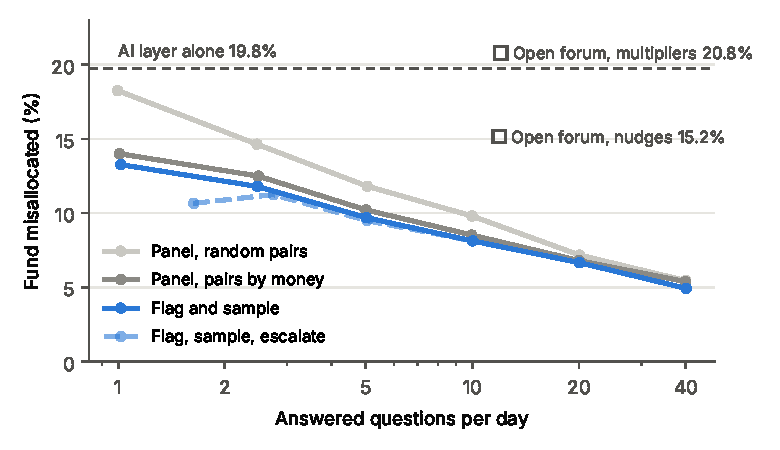
\includegraphics[width=0.85\linewidth]{frontier.pdf}
  \caption{Misallocation by attention. At 5 to 10 answered questions a day, flag and sample leaves 9.7\% to 8.1\% of the fund misallocated, against 19.8\% for the engine alone.}
  \label{fig:frontier}
\end{figure}

\begin{figure}[t]
  \centering
  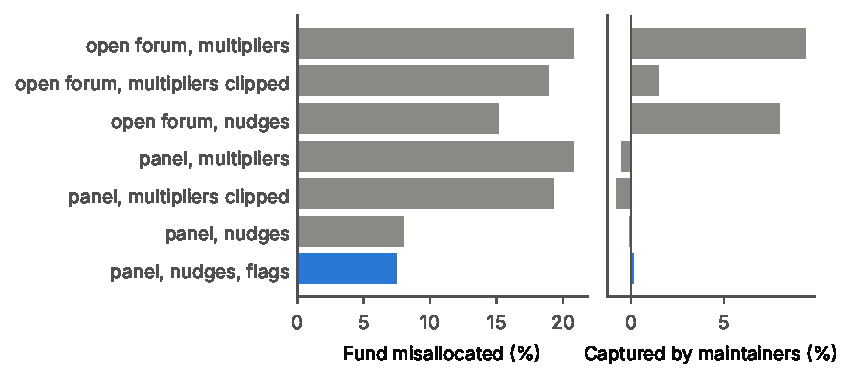
\includegraphics[width=0.85\linewidth]{steering.pdf}
  \caption{Seven designs at about 12 answered questions a day. Recusal removes capture; fixed-step answers beat multipliers.}
  \label{fig:steering}
\end{figure}

Figure~\ref{fig:frontier} shows the frontier, and Figure~\ref{fig:steering} compares designs at equal attention.
Every design that lets maintainers answer about their own project hands them between 1.5\% and 9.4\% of the fund, and every design with recusal keeps capture within noise of zero.
With the multiplier inflation measured in the trial, multiplier designs do not improve on the engine, even when clipped and recused.

\section{Related Work}
Iterative Local Voting steers a point in a continuous space by local moves of randomly sampled voters, with a stochastic-gradient analysis~\citep{garg2017ilv}; we add volunteers with a stake, flags as an agenda, a fixed step that tracks change, recusal, escalation, and an engine.
The geometric median is not even approximately strategyproof but is asymptotically~$\alpha$-strategyproof~\citep{elmhamdi2023median}, and moving-phantom mechanisms aggregate budget proposals truthfully in a one-shot setting~\citep{freeman2021budget}.
With costly voluntary voting, turnout follows intensity~\citep{krishna2015majority}, and strategyproof responsive rules with participation costs leave a single participant at an extreme~\citep{muller2020participation}; both motivate separating voluntary attention from the verdict.
Decentralized courts draw jurors at random once a party raises a dispute~\citep{lesaege2019kleros}, and AI control spends a limited budget of trusted human review where a monitor is suspicious~\citep{greenblatt2024control}.
Active pair selection for crowdsourced ranking chooses questions under a budget~\citep{chen2013crowdbt}, and step sizes can follow sign changes~\citep{kesten1958accelerated} or balance drift against noise~\citep{cutler2021drift}.
Collective control of AI has been framed as social choice across the machine learning pipeline~\citep{bachmann2026collective}, and policies that require human oversight of algorithms often fail in practice~\citep{green2022oversight}.

\section{Outlook}
Three directions follow.
First, an adversarial engine that chooses what members see, against which random spot checks act as an audit.
Second, stirring the constitution itself, with speed parameters tuned freely and destination parameters reserved for larger panels.
Third, a field study of question formats, to measure whether showing the current amounts removes inflation.

\bibliographystyle{plainnat}
\bibliography{refs}
\end{document}
